\section{Máquina de Boltzmann}

\begin{frame}
  \justifying%
  \begin{alertblock}{}
    \centering
    Máquina de BOLTZMANN
  \end{alertblock}
\end{frame}

\begin{frame}{Máquina de Boltzmann}%
  \justifying%
  Rede estocástica com $\omega_{ij} = \omega_{ji}$.
  \\~\\
  Possui dois tipos de unidades distintas: unidades \textbf{visíveis} e unidades \textbf{escondidas}.
  \\~\\
  \textbf{Visíveis}: ligadas ao meio externo; correspondem às variáveis do problema.
  \\~\\
  \textbf{Escondidas}: não tem ligação do o meio externo; determinam a relação entre as variáveis do problema.
\end{frame}

\subsection{Esquema}
\begin{frame}{Arquitetura de BMs}%
  \begin{figure}[h]{}%
    \label{fig:bm-diagram-1}%
    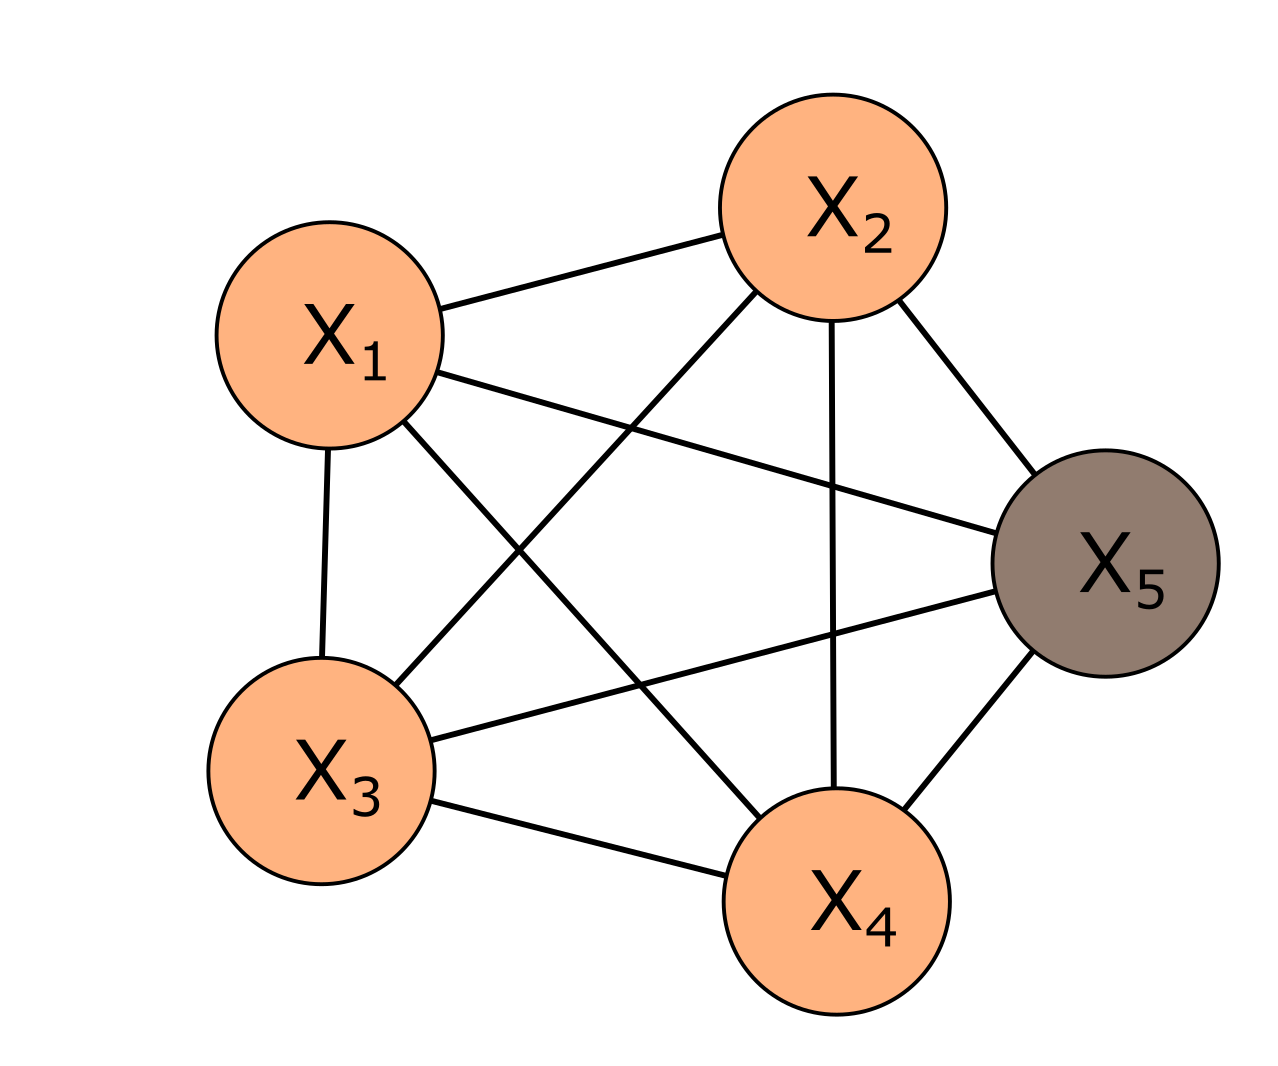
\includegraphics[scale=0.5]{images/bm_1.png}
    \caption{Diagrama de uma máquina de Boltzmann.}
  \end{figure}
\end{frame}

\begin{frame}{Arquitetura de BMs}%
  \begin{figure}[h]{}%
    \label{fig:bm-diagram-2}%
    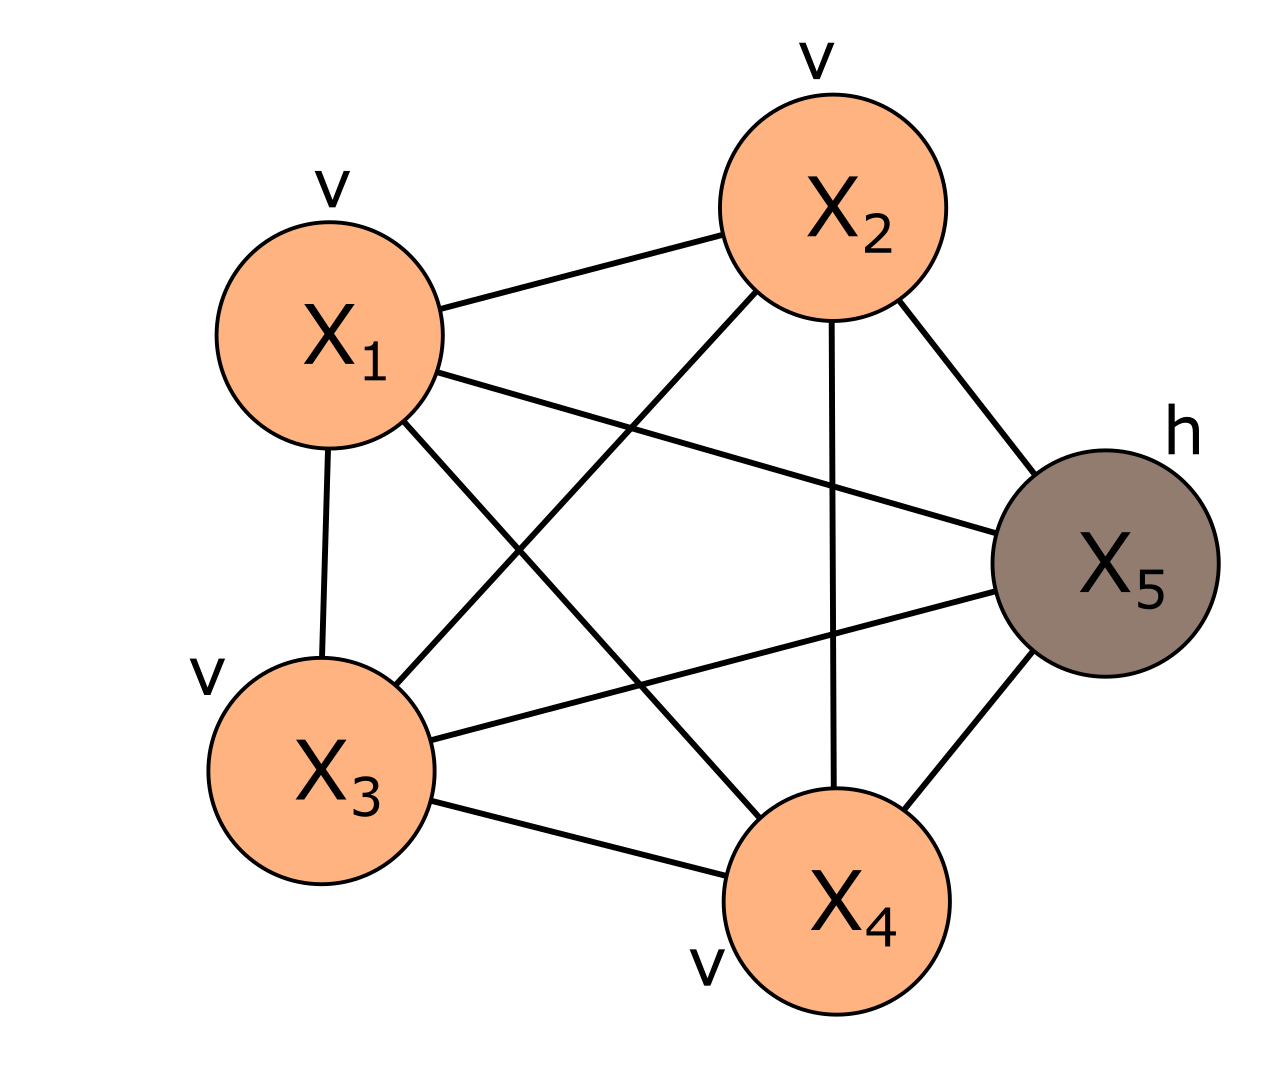
\includegraphics[scale=0.5]{images/bm_2.png}
    \caption{Diagrama de uma máquina de Boltzmann; unidades mais claras são as visíveis, e unidades mais escuras, as escondidas.}
  \end{figure}
\end{frame}

\subsection{Considerações}
\begin{frame}{O sistema}%
  \justifying%
  \onslide<1->{%
  Vamos considerar que temos uma rede com $N$ unidades visíveis, e $K$ unidades escondidas, }
  \onslide<2->{%
  em que as unidades visíveis estão no estado $v$, e as escondidas, no estado $h$.} 
  \\~\\
  \onslide<3->{%
  Temos $2^{(N + K)}$ possibidades de estados em que a rede pode ser encontrada.
  }
  \\~\\
  \onslide<4->{%
  Uma unidade $\mathrm{x}_{i} = x_{i}$, sendo que $x_{i} \in \{0, 1\}$. 
  }
\end{frame}

\subsection{Aprendizagem}%
\begin{frame}{Objetivo da Máquina de Boltzmann}%
  \justifying%
  \onslide<1->{%
  Na máquina de Boltzmann fazemos o ajuste das conexões $\omega_{ij}$ para termos um certo estado nas unidades visíveis com uma distribuição de probabilidade desejada.
  \\~\\
  Se precisamos determinar as conexões $\omega_{ij}$, precisamos de um mecanismo para atualizar os pesos, temos que resolver:
  }
  \onslide<2->{%
  \begin{equation}%
    \label{eq:omega-learning}
    \omega^{(final)}_{ij} = \omega^{(inicial)}_{ij} + \Delta \omega_{ij}.
  \end{equation}
  }
  \\~\\
  \onslide<3->{%
  Lembrando que os pesos são ajustados baseados nos exemplos de treinamento que a rede recebe.  
  }
\end{frame}

\begin{frame}{Grandezas Importantes}%
  \justifying%
  Energia para rede com unidades visíveis no estado $v$, e escondidas, no estado $h$:
  \begin{equation}%
    \label{eq:bm-energy}
    H_{vh} = -\frac{1}{2} \sum_{i} \sum_{j} \omega_{ij} x^{(vh)}_{i} x^{(vh)}_{j} - \sum_{i} \phi_{i} x^{(vh)}_{i}.
  \end{equation}
  \\~\\
  Podemos calcular a soma de todos os possíveis estados da rede pela função partição:
  \begin{equation}%
    \label{eq:bm-partition}
    Z = \sum_{u} \sum_{k} e^{(-\beta H_{uk})}.
  \end{equation}
\end{frame}

\begin{frame}{Grandezas Importantes}%
  A probabilidade $P_{v}$ de achar as unidades visíveis de uma máquina de Boltzmann em um determinado estado $v$, é
  \begin{equation}%
    \label{eq:bm-prob-marg}%
    P_{v} = \sum_{h} \frac{1}{Z} e^{(-\beta H_{vh})}.
  \end{equation}
  \\~\\
  Também pode ser escrito como
  \begin{equation}%
    \label{eq:bm-prob-marg2}
    P_{v} = \frac{\sum_{h} e^{-\beta H_{vh}}}{\sum_{u} \sum_{k} e^{-\beta H_{uk}}}.
  \end{equation}
\end{frame}

\begin{frame}{Entropia Relativa - Divergência Kullback-Leibler}%
  \justifying%
  Se temos duas distribuições de probabilidade distintas, por exemplo, $P$ e $R$, sobre um mesmo espaço de estados, podemos calcular a diferença entre estas distribuições pela entropia relativa, $E$, (ou divergência de Kullback-Leibler, $D_{KL}(R||P)$).
\end{frame}

\begin{frame}{Entropia Relativa - Divergência Kullback-Leibler}%
  \justifying%
  Com as máquinas de Boltzmann queremos determinar a probabilidade $P_{v}$ de achar as unidades visíveis em determinado estado $v$, como mostra a equação~(\ref{eq:bm-prob-marg}). Porém para este estado temos uma probabilidade deseja $R_{v}$.
  \begin{equation}%
    \label{eq:bm-entropy}
    E = \sum_{v} R_{v} \ln \left[\frac{R_{v}}{P_{v}} \right]
  \end{equation}
\end{frame}

\begin{frame}{Atualização de $\Delta \omega_{ij}$}%
  \justifying%
  Usamos a nossa entropia relativa como função custo.
  \\~\\
  Pelo método do grandiente descendente, podemos calcular $\Delta \omega_{ij}$,
  \begin{equation}%
    \label{eq:omega-delta}
    \Delta \omega_{ij} = -\eta \frac{\partial E}{\partial \omega_{ij}},
  \end{equation}
  onde $\eta$ é a taxa de aprendizagem.
  \\~\\
  $E(P_{v})$; $P_{v}(H_{vh})$; $H_{vh}(\omega_{ij})$.
\end{frame} 

\begin{frame}{Atualização de $\Delta \omega_{ij}$}%
  \justifying%
  Por simplificação, vamos considerar que a função de energia para a rede no estado $v$ e $h$ é dada apenas pela correlação entre as unidades (primeiro termo da equação~(\ref{eq:bm-energy})):
  \begin{equation}%
    \label{eq:bm-energy-simple}
    H_{vh} = -\frac{1}{2} \sum_{i} \sum_{j} \omega_{ij} x^{(vh)}_{i} x^{(vh)}_{j}  
  \end{equation}
\end{frame}

\begin{frame}{Atualização de $\Delta \omega_{ij}$}%
  \justifying%
  Para se determinar $\Delta \omega_{ij}$, temos que passar por uma série de derivações$\dots$
  \begin{align}%
    \phantom{\frac{\partial P_{v}}{\partial \omega_{ij}}}%
    & \onslide<1->
    \begin{aligned}
      \mathllap{\Delta \omega_{ij}} & = \eta \sum_{v} \frac{R_{v}}{P_{v}} \frac{\partial P_{v}}{\partial \omega_{ij}} 
    \end{aligned} \\ }
    & \onslide<2->{%
    \label{eq:bm-prob-deriv-1}%
    \begin{aligned}
        \mathllap{\frac{\partial P_{v}}{\partial \omega_{ij}}} & = \beta \left[-\sum_{h} \frac{e^{-\beta H_{vh}}}{Z} \frac{\partial H_{vh}}{\partial \omega_{ij}} + \sum_{h} \frac{e^{-\beta H_{vh}}}{Z} \sum_{u} \sum_{k} \frac{e^{-\beta H_{uk}}}{Z} \frac{\partial H_{uk}}{\partial \omega_{ij}} \right] 
    \end{aligned} \\ }
    & \onslide<3->{%
    \label{eq:energy-deriv-1}
    \begin{aligned}
        \mathllap{\frac{\partial H}{\partial \omega_{ij}}} & = - x_{i} x_{j} 
    \end{aligned} }
  \end{align}
\end{frame}

\begin{frame}{Atualização de $\Delta \omega_{ij}$}%
  \justifying%
  \onslide<1->{%
  Com as devidas substituições na equação~(\ref{eq:bm-prob-deriv-1}), temos
  \begin{equation}%
    \label{eq:bm-prob-deriv-2}
    \frac{\partial P_{v}}{\partial \omega_{ij}} = \beta \left[\sum_{h} P_{vh} x^{(vh)}_{i} x^{(vh)}_{j} - P_{v} \sum_{u} \sum_{k} P_{uk} x^{(uk)}_{i} x^{(uk)}_{j} \right] 
  \end{equation}
  \\~\\
  }
  \onslide<2->{%
  No segundo termo, temos o valor médio da correlação entre as unidades $i$ e $j$, que é dado por
  \begin{equation}%
    \label{eq:valor-medio}%
    \langle x_{i} x_{j} \rangle = \sum_{u} \sum_{k} P_{uk} x^{(uk)}_{i} x^{(uk)}_{j}
  \end{equation}
  }
\end{frame}

\begin{frame}{Atualização de $\Delta \omega_{ij}$}%
  \justifying%
  Substituindo as equações~(\ref{eq:bm-prob-deriv-2}) e (\ref{eq:valor-medio}) em (\ref{eq:omega-deriv-1}):
  \begin{equation}%
    \label{eq:omega-deriv-2}%
    \Delta \omega_{ij} = \eta \beta \left[ \sum_{v} \sum_{h} R_{v} \frac{P_{vh}}{P_{v}} x^{(vh)}_{i} x^{(vh)}_{j} - \sum_{v} R_{v} \langle x_{i} x_{j} \rangle \right]
  \end{equation}
  \\~\\
  Considerando o probabilidade condicional 
  \begin{equation}%
    \label{eq:prob-condic}%
    P_{h|v} = \frac{P_{vh}}{P_{v}},
  \end{equation}
  podemos rearranjar o primeiro termo de~(\ref{eq:omega-deriv-2}),
  \begin{equation}%
    \label{eq:omega-deriv-term1}%
    \sum_{v} R_{v} \sum_{h} P_{h|v} x^{(vh)}_{i} x^{(vh)}_{j} = \sum_{v} R_{v} \langle x_{i} x_{j} \rangle^{(v)} = \langle \langle x_{i} x_{j} \rangle^{(v)} \rangle
  \end{equation}
\end{frame}

\begin{frame}{$\Delta \omega_{ij}$}%
  \justifying%
  Por último, temos que o termo responsável pela atualização dos pesos é
  \begin{equation}%
    \label{eq:omega-deriv-final}
    \Delta \omega_{ij} = \eta \beta \left[ \langle \langle x_{i} x_{j} \rangle^{(v)} \rangle_{fixo} - \langle x_{i} x_{j} \rangle_{llivre}  \right]
  \end{equation}
  \\~\\
  O primeiro termo corresponde ao valor médio de acordo com a distribuição de probabilidade $R_{v}$ do valor médio das correlações entre as unidades $i$ e $j$ quando as unidades visíveis estão no estado fixo $v$.
  \\~\\
  O segundo termo corresponde a média da correlação entre as unidades $i$ e $j$ para todas as combinações possíveis dos estados $v$ e $h$ do sistema.
\end{frame}

